\documentclass{beamer}
\usepackage{textpos}
\setlength{\TPHorizModule}{1cm} % Horizontale Einheit
\setlength{\TPVertModule}{1cm} % Vertikale Einheit
\usepackage{lmodern}
\usepackage{xcolor}
\usepackage{algpseudocode}
\usepackage{amsmath}
\usepackage{tcolorbox}
\usepackage{tikz}
\usepackage{soul}
\usepackage[update,prepend]{epstopdf}
\usepackage{adjustbox}
\usepackage{setspace}
\usepackage[font={scriptsize}, justification=centering]{caption}
\usepackage[font={color=black}]{subcaption}
\usepackage{ellipsis}
\usetikzlibrary{decorations.pathmorphing,calc}
\usetikzlibrary{decorations.pathreplacing}
\usetikzlibrary{positioning}
\usepackage{chemarrow}
\usepackage{slashbox}
\usepackage[ruled,vlined,linesnumbered]{algorithm2e}
\usepackage{siunitx}
\usepackage{relsize}
\usepackage{3dplot}
\usepackage{threeparttable}
\usetikzlibrary{fit}
\usepackage[utf8]{inputenc}
\usepackage[upright]{fourier}
\usetikzlibrary{matrix,arrows,decorations.pathmorphing}
\usepackage{xparse}
\usepackage[nomessages]{fp}% http://ctan.org/pkg/fp
\usetikzlibrary{calc}
\usepackage{breqn} %for dmath
\usepackage{hyperref} 
\usepackage{arydshln}
\usetikzlibrary{shapes,fit}
\definecolor{univred}{rgb}{0.7, 0.0, 0.0}
\definecolor{drkgreen}{rgb}{0,0.26,0.15}
\definecolor{aureolin}{rgb}{0.99,0.93,0.0}
\DeclareMathOperator*{\argmax}{argmax}
%
%
\newcolumntype{C}[1]{>{\centering\let\newline\\\arraybackslash\hspace{0pt}}m{#1}}
\setbeamertemplate{background canvas}{%
    {\color{univred}\noindent\makebox[\paperwidth]{\rule{\paperwidth}{2.5ex}}
}}
\setbeamertemplate{frametitle}{\color{black}\bfseries\vskip2ex\insertframetitle\par\vskip-6pt\hrulefill}
\addtobeamertemplate{frametitle}{}{%
%CMU logo in header
    \begin{textblock*}{100mm}(0.87\textwidth,-1.425cm)
        \includegraphics[height=1.5cm,width=1.9cm,keepaspectratio]{cm_logo}
    \end{textblock*}
%ECE logo in footer
    \begin{textblock*}{10mm}(-.8cm,7.5cm)
        \includegraphics[height=2cm,width=2.5cm,keepaspectratio]{ece}
    \end{textblock*}
}
\addtobeamertemplate{footnote}{}{\vspace{2ex}}
\setbeamercolor*{item}{fg=black}
\setbeamertemplate{footline}[page number]{}
\setbeamercolor{page number in head/foot}{fg=univred}

\makeatletter
\newcommand{\defhighlighter}[3][]{%
    \tikzset{every highlighter/.style={color=#2, fill opacity=#3, #1}}%
}

\defhighlighter{yellow}{.5}
\newcommand{\highlight@DoHighlight}{
    \fill [ decoration = {segment length=13pt}
        , outer sep = -15pt, inner sep = 0pt, decorate
    , every highlighter, this highlighter ]
    ($(begin highlight)+(0,8pt)$) rectangle ($(end highlight)+(0,-1pt)$) ;
}

\newcommand{\highlight@BeginHighlight}{
    \coordinate (begin highlight) at (0,0) ;
}

\newcommand{\highlight@EndHighlight}{
    \coordinate (end highlight) at (0,0) ;
}

\newdimen\highlight@previous
\newdimen\highlight@current

\DeclareRobustCommand*\highlight[1][]{%
    \tikzset{this highlighter/.style={#1}}%
    \SOUL@setup
  %
    \def\SOUL@preamble{%
        \begin{tikzpicture}[overlay, remember picture]
            \highlight@BeginHighlight
            \highlight@EndHighlight
        \end{tikzpicture}%
    }%
  %
    \def\SOUL@postamble{%
        \begin{tikzpicture}[overlay, remember picture]
            \highlight@EndHighlight
            \highlight@DoHighlight
        \end{tikzpicture}%
    }%
  %
    \def\SOUL@everyhyphen{%
        \discretionary{%
            \SOUL@setkern\SOUL@hyphkern
            \SOUL@sethyphenchar
            \tikz[overlay, remember picture] \highlight@EndHighlight ;%
        }{%
        }{%
            \SOUL@setkern\SOUL@charkern
        }%
    }%
  %
    \def\SOUL@everyexhyphen##1{%
        \SOUL@setkern\SOUL@hyphkern
        \hbox{##1}%
        \discretionary{%
            \tikz[overlay, remember picture] \highlight@EndHighlight ;%
        }{%
        }{%
            \SOUL@setkern\SOUL@charkern
        }%
    }%
  %
    \def\SOUL@everysyllable{%
        \begin{tikzpicture}[overlay, remember picture]
            \path let \p0 = (begin highlight), \p1 = (0,0) in \pgfextra
            \global\highlight@previous=\y0
            \global\highlight@current =\y1
        \endpgfextra (0,0) ;
        \ifdim\highlight@current < \highlight@previous
        \highlight@DoHighlight
        \highlight@BeginHighlight
        \fi
    \end{tikzpicture}%
    \the\SOUL@syllable
    \tikz[overlay, remember picture] \highlight@EndHighlight ;%
}%
\SOUL@
}
\makeatother

\title{\color{univred} A Comparison of Antenna Placement Algorithms}
\author{Abhinav Jauhri}
\date{\today}
\begin{document}
\begin{frame}
    \color{univred}
    \titlepage
\end{frame}

\begin{frame}{Contributions}
\begin{itemize} \itemsep1.5em
        \item Formulation of the antenna placement problem
        \item Evaluation of standard stochastic algorithms on a real-world problem
        \item Able to achieve global optimum with as low as \textbf{25\% evaluations} of search space
    \end{itemize}
    \vspace{5mm}
\end{frame}


\begin{frame}{Minimize Difference in Radiation Pattern}
    Pattern defines the ratio of energy radiated and input energy in a particular direction. For each antenna $A_i$:
    \begin{tcolorbox}[colback=green!5]
        \begin{equation} \label{eq:rp}
            F_{RP} = \sum_{i=1}^n\sum_{\theta=0}^\pi\sum_{\phi=0}^{2\pi}
            \left( FSG_i(\theta,\phi) - ISG_i(\theta,\phi) \right) ^2,
        \end{equation}
    \end{tcolorbox}
    where
    \begin{itemize}
            \small
        \item $\theta, \phi$ spherical coordinates
        \item $FSG(\cdot)$ returns free-space gain pattern  
        \item $ISG(\cdot)$ returns in-situ gain pattern
    \end{itemize}

    \tdplotsetmaincoords{60}{110}
    \pgfmathsetmacro{\rvec}{.8}
    \pgfmathsetmacro{\thetavec}{30}
    \pgfmathsetmacro{\phivec}{60}
    \hspace{.6\textwidth}
    \begin{tikzpicture}[scale=1.8,tdplot_main_coords]
        \tikzstyle{every node}=[font=\tiny]
        \coordinate (O) at (0,0,0);
        \tdplotsetcoord{P}{\rvec}{\thetavec}{\phivec}
        \draw[thick,->] (0,0,0) -- (1,0,0) node[anchor=north east]{$x$};
        \draw[thick,->] (0,0,0) -- (0,1,0) node[anchor=north west]{$y$};
        \draw[thick,->] (0,0,0) -- (0,0,1) node[anchor=south]{$z$};
        \draw[-stealth,color=red] (O) -- (P);
        \draw[dashed, color=red] (O) -- (Pxy);
        \draw[dashed, color=red] (P) -- (Pxy);
        \tdplotdrawarc{(O)}{0.2}{0}{\phivec}{anchor=north}{$\phi$}
        \tdplotsetthetaplanecoords{\phivec}
        \tdplotdrawarc[tdplot_rotated_coords]{(0,0,0)}{0.5}{0}{\thetavec}{anchor=south west}{$\theta$}
        \draw[dashed,tdplot_rotated_coords] (\rvec,0,0) arc (0:90:\rvec);
        \draw[dashed] (\rvec,0,0) arc (0:90:\rvec);
    \end{tikzpicture}
\end{frame}

\begin{frame}{Radiation Pattern}
    \begin{columns}
        \begin{column}{0.5\linewidth}
            \begin{figure}
                \vspace*{-2cm}
                \caption*{Free-space pattern without platform or other antennas}
                \centering
                \includegraphics[width=4cm]{../paper/FIG/free_space.png}
            \end{figure}
        \end{column}
        \begin{column}{0.5\linewidth}
\begin{overlayarea}{\textwidth}{\textheight}
            \begin{figure}
                \vspace*{-0.7cm}
                \begin{subfigure}{\columnwidth}
                    \centering
                        \caption*{\tiny {Random in-situ pattern with platform and antennas}}%
                        \includegraphics[width=0.5\columnwidth,height=0.5\columnwidth]{../paper/FIG/rand.png}
                \end{subfigure}\\\vfill
                \only<2>{
                \begin{subfigure}{\columnwidth}
                    \centering
                    \caption*{\tiny {Best in-situ pattern with platform and antennas similar to free-space pattern}}%
                    \includegraphics[width=0.5\columnwidth, height=0.5\columnwidth]{../paper/FIG/best.png}%
                \end{subfigure}\hfill\\}%
            \end{figure}
        \end{overlayarea}
        \end{column}
    \end{columns}
\end{frame}
\begin{frame}{GA with different mutation rates}
    \begin{figure}
        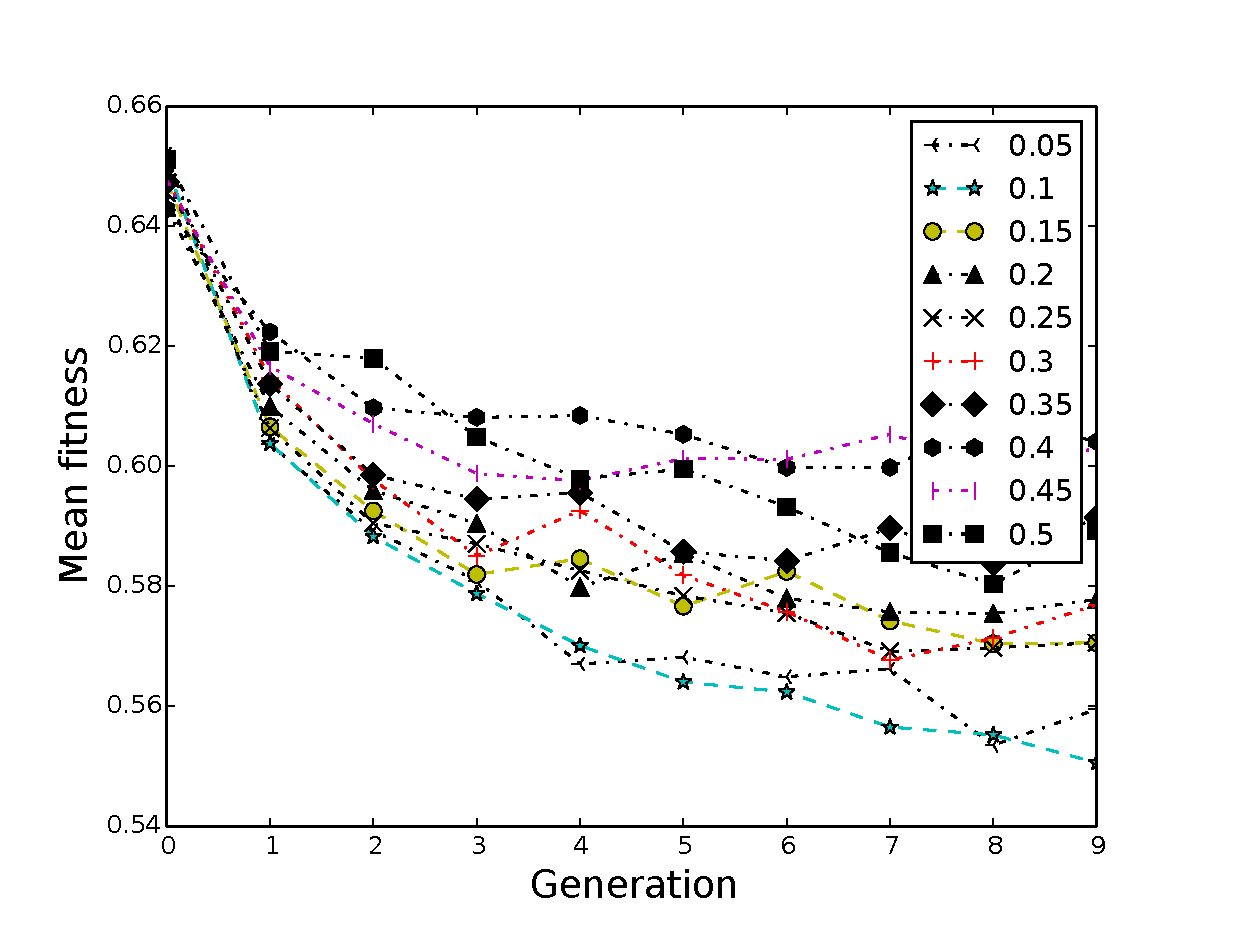
\includegraphics[scale=0.45]{../paper/FIG/ga_mut.eps}
    \end{figure}
\end{frame}

\begin{frame}{Equivalence of fitness to efficiency}
    \small For a particular test case, fitness change of $0.01$ is equivalent to either the corresponding value under expected gain ($\mathbb E_g$) column, or difference in coupling ($\Delta_c$).
    \begin{table}
        \centering
        \begin{threeparttable}
            \begin{tabular}{|C{1cm}|C{2.5cm}|C{2.5cm}|} \hline
                ID& $\mathbb E_g$ & $\Delta_{c}$ (dB) \\ \hline
                tc1 & 872.277 & 0.5474 \\ \hline
                tc2 & 862.082 & 1.3034 \\ \hline
                tc3 & 861.845 & 1.5180 \\ \hline
                tc4 & 871.049 & 0.5693 \\
                \hline\end{tabular}
        \end{threeparttable}
    \end{table}
    \tiny
    $\mathbb E_g = \frac{1}{N \cdot m} \sum_{i}^m F_{RP}(A_i),$
    where $N = \;\mid \theta \mid \cdot \mid \phi \mid$
\end{frame}

\end{document}
